\documentclass[12pt]{article}
\usepackage{amsmath}
%\usepackage{fullpage}
\usepackage[top=1in, bottom=1in, left=0.8in, right=1in]{geometry}
\usepackage{multicol}
\usepackage{wrapfig}
\usepackage{graphicx}
\usepackage{float}
\usepackage{listings}
\usepackage{enumerate}
\lstset{language=Java,
	basicstyle={\small\ttfamily},
	columns=flexible,
	belowskip=0mm}

\setlength{\columnsep}{0.1pc}

\title{ME573 Homework Set \# 7}
\author{Alexander Swenson -- \texttt{aaswenson@wisc.edu}}
\date{\today}
\begin{document}
	
	\maketitle
	
	\vspace{-0.3in}
	\noindent
	\rule{\linewidth}{0.4pt}
	
	\noindent
	
	%%%%%%%%%%%%%%%%%%%%%%%%%%%%%%%%%%%%%%%%%%%%%%%%%%%%%%%%%%%%%%%%%%%%%%%%%%%%%%%%
	% Problems 1
	
	\section{Introduction}
	
	\noindent This coding assignment involved modeling 2D heat diffusion with the Alternating Direct Implicit Method (ADI) algorithm.	The algorithm was implemented in MATLAB (see attached code).
	
	%%%%%%%%%%%%%%%%%%%%%%%%%%%%%%%%%%%%%%%%%%%%%%%%%%%%%%%%%%%%%%%%%%%%%%%%%%%%%%%%
	
	\section{Part A}
	
	\noindent The $L_{\inf}$ norm was calculated between the initial conditions ans the exact solution (evaluated at t=0). The norm was: 1.2053e-05
	
	\begin{figure}[H]
		\centering
		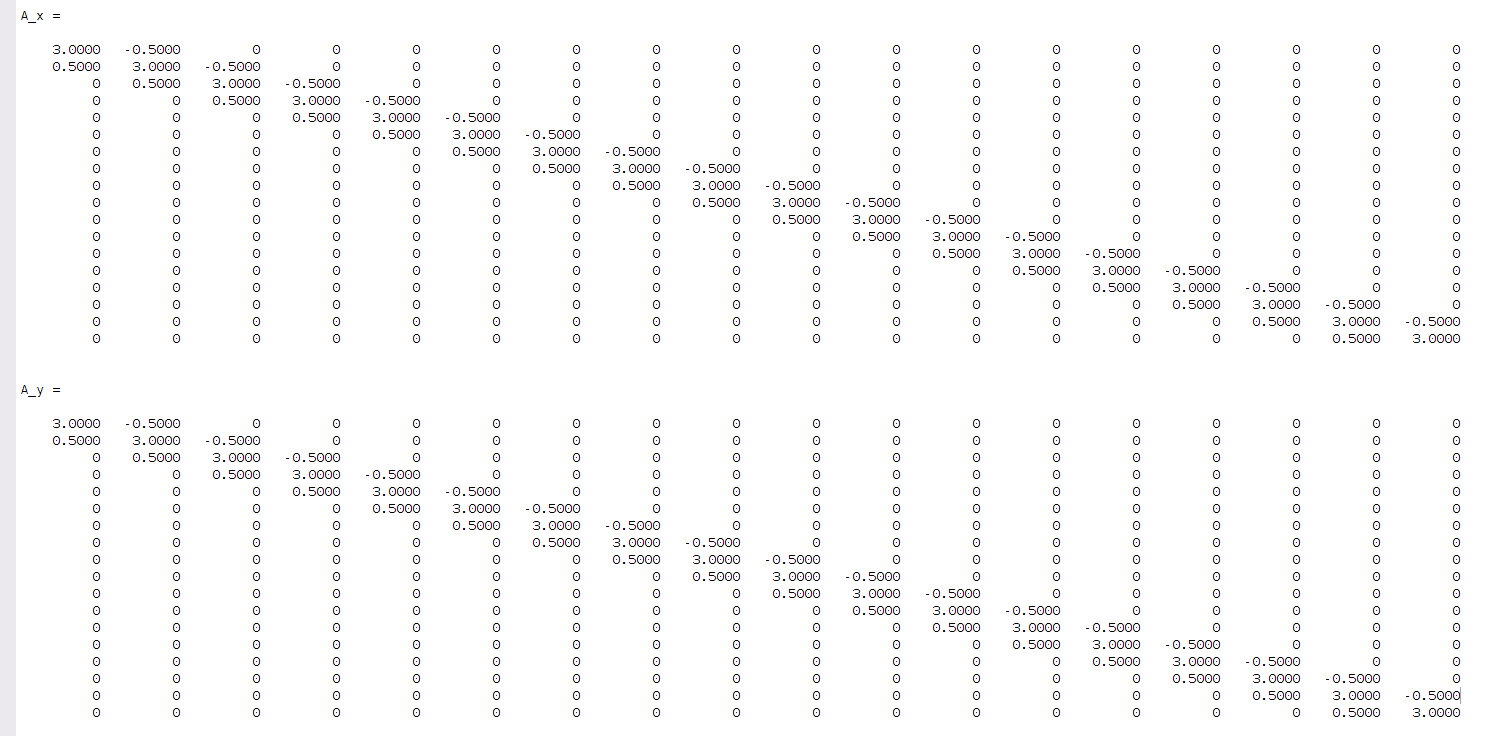
\includegraphics[height=3.75in]{matrixAxAy.png}
		\label{fig:problem2_plot}
	\end{figure}
	%%%%%%%%%%%%%%%%%%%%%%%%%%%%%%%%%%%%%%%%%%%%%%%%%%%%%%%%%%%%%%%%%%%%%%%%%%%%%%%%
	
		\section{Part C}
		
		\noindent The following figures contain the b vectors used to solve the problem. They are the vectors used in the first time step (1-a) and (1-b).
		
		\begin{figure}[H]
			\centering
			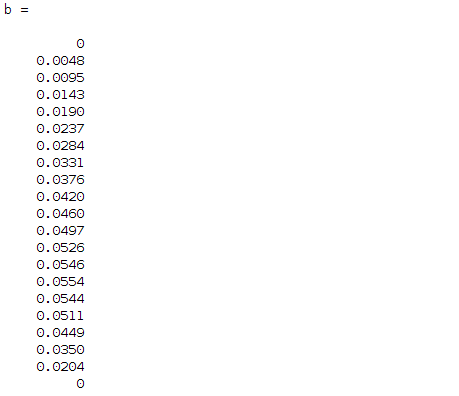
\includegraphics[height=3.75in]{b_mat_1.png}
			\label{fig:bmat1}
		\end{figure}
		
		\begin{figure}[H]
			\centering
			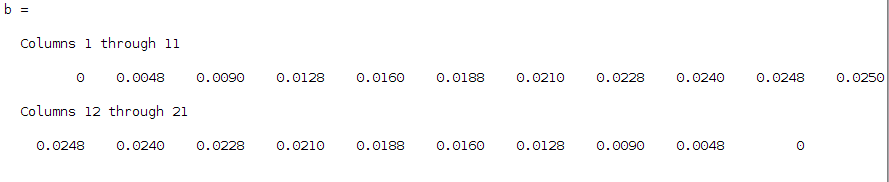
\includegraphics[height=1.5in]{b_mat_2.png}
			\label{fig:bmat2}
		\end{figure}
		
	%%%%%%%%%%%%%%%%%%%%%%%%%%%%%%%%%%%%%%%%%%%%%%%%%%%%%%%%%%%%%%%%%%%%%%%%%%%%%%%%
			
	\section{Part D}
	
	\noindent The following Figure \ref{fig:error} shows the error between the exact solution and the ADI method at the end of the time steps.
	
	\begin{figure}[H]
		\centering
		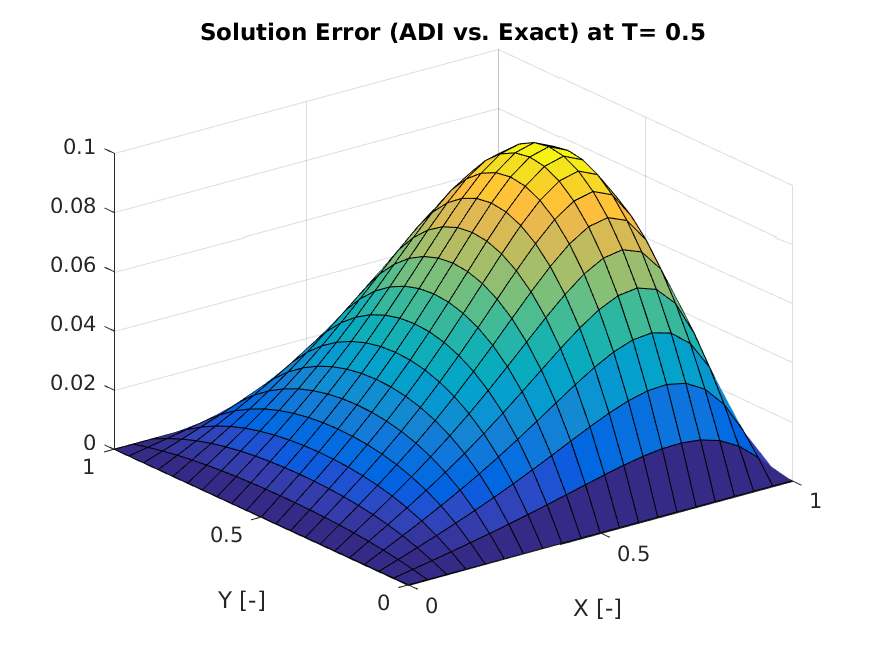
\includegraphics[height=3.75in]{solution_error.png}
		\label{fig:error}
	\end{figure}	
	
	
	
	
	
\end{document}